%%%%%%%%%%%%%%%%%%%%%%%%%%%%%%%%%%%%%%%%%%%%%%%%%%%%%%%%%%%%%%%%%%%%%%%%
% Springer LNCS class (llncs.cls, v2.20)
%%%%%%%%%%%%%%%%%%%%%%%%%%%%%%%%%%%%%%%%%%%%%%%%%%%%%%%%%%%%%%%%%%%%%%%%
\documentclass{llncs}

\usepackage{graphicx}
\usepackage{amsmath}
\usepackage{amssymb}
\usepackage{booktabs}
\usepackage{array}
\newcolumntype{L}[1]{>{\raggedright\arraybackslash}p{#1}}
\usepackage{tikz}
\usetikzlibrary{arrows.meta,positioning}

\begin{document}
\pagestyle{plain}

\title{Learning Which Item to Evict Inside an Adaptive Replacement Cache}
\titlerunning{Learning Which Item to Evict Inside ARC}

\author{Yash Laxman \and R Ajay Kumar \and Kritharth B Shetty \and Pooja J Naik}

\institute{Department of Computer Science and Engineering,\\
Sahyadri College of Engineering \& Management, Mangaluru, India}

\maketitle

\begin{abstract}
Every cache has to decide which item to remove when it runs out of space. Classic rules such as LRU and LFU each work well on some workloads and poorly on others. ARC improves on them by balancing recency against frequency, but once it has picked a list to shrink it always removes the oldest item in that list. This chapter proposes TIDE, a design that keeps ARC exactly as it is and hands the final eviction choice to a deep feedforward neural network trained continually on live traffic. The network is the central contribution of this work: a three-hidden-layer architecture that turns twelve recency, frequency and periodicity features into a single reuse-time score, trained end to end by backpropagation with no offline dataset and no reward shaping. It learns from delayed labels that the request stream produces on its own, replayed through an experience buffer in the style of deep reinforcement learning systems, and it may also decide not to cache a new item at all. We describe the network's architecture and training procedure in detail, explain why it should help on looping and phase-based workloads and why it cannot help on purely random traffic, show how a shadow copy of ARC limits the damage when the network is wrong, and set out a plan for testing these expectations.

\keywords{Deep learning \and Neural networks \and Cache replacement \and Adaptive replacement cache \and Online learning \and Eviction policy}
\end{abstract}

\section{Introduction}
\label{sec:intro}

A cache keeps a small number of items close at hand so that repeated requests can be served quickly. When the cache is full and a new item arrives, something has to go. The rule that makes this choice is the replacement policy, and it decides the hit rate: the share of requests the cache can answer without going to slower storage. Even a few points of hit rate can matter a great deal, because every miss costs a disk read, a database query or a network trip.

The best possible rule has been known for a long time. Belady showed that a cache should remove the item that will be needed furthest in the future~\cite{belady1966}. Real systems cannot see the future, so they guess. LRU guesses that recently used items will be used again soon. LFU guesses that popular items will stay popular. Each guess holds on some workloads and fails on others.

Learned policies try to replace these fixed guesses with a model trained on real traffic~\cite{song2020,liu2020}. In practice they tend to throw away the heuristic they replace, they add cost to every decision, and they can do much worse than the old rule when the model is wrong. We take a narrower path. ARC~\cite{megiddo2003} already does one thing well: it decides whether the recency side or the frequency side of the cache should shrink. It does a second thing poorly: inside the chosen side it always removes the oldest item. TIDE keeps the first decision and hands the second to a deep neural network.

The network is deliberately the centrepiece of this chapter. It is a three-hidden-layer feedforward architecture, deep rather than shallow, trained continually on live traffic with no offline dataset, no hand-labelled examples and no reward shaping of the kind reinforcement learning needs. This chapter makes four contributions. It frames eviction as ranking a few candidates by how soon they will return. It presents a complete deep learning based design built on that idea, including the network's architecture, its input representation and its training procedure. It gives simple arguments for how the design should behave, including its cost and how far it can fall behind ARC. Finally, it turns those arguments into predictions and a plan for testing them.

\section{Related Work}
\label{sec:background}

\subsection{Belady's Rule}

Belady's rule removes the item whose next request is furthest away, and no other demand paging policy can have fewer misses on the same sequence~\cite{belady1966}. It is used as a yardstick. A common way to report results is a normalised hit rate, where 0 means no better than LRU and 1 means as good as Belady's rule. When requests are drawn at random from a fixed set of popularities, the best rule that does not know the future is simply to keep the most popular items~\cite{aho1971}.

\subsection{Classic Policies}

Table~\ref{tab:heuristics} lists the classic policies that matter most here. Each one relies on a single idea about the workload, and each has a case where that idea breaks.

\begin{table}[htbp]
\centering
\caption{Classic replacement policies.}
\label{tab:heuristics}
\begin{tabular}{L{2.2cm}L{4.2cm}L{4.7cm}}
\toprule
Policy & Main signal & Where it struggles \\
\midrule
LRU & Time since last use & Scans and loops longer than the cache \\
LFU & Number of uses & Holds on to items that are no longer popular \\
2Q~\cite{johnson1994} & Trial queue, then LRU & Queue sizes are fixed in advance \\
LIRS~\cite{jiang2002} & Gap between uses & Extra bookkeeping and tuning \\
ARC~\cite{megiddo2003} & Recency and frequency lists & Always removes the oldest item of a list \\
S3-FIFO~\cite{yang2023} & Small and main FIFO queues & No view of when an item returns \\
SIEVE~\cite{zhang2024} & FIFO with a visited bit & Only a yes or no view of reuse \\
\bottomrule
\end{tabular}
\end{table}

\subsection{How ARC Works}

ARC splits the cache into two lists. $T_1$ holds items seen once recently and $T_2$ holds items seen at least twice. It also remembers the keys of recently removed items in two ghost lists, $B_1$ and $B_2$, without keeping their data. If a request hits a ghost list, ARC takes it as a sign that it shrank the wrong list, and it moves a target size $p$ in the other direction. When space is needed, ARC removes an item from $T_1$ if $T_1$ is larger than $p$ and from $T_2$ otherwise.

This choice of list is ARC's strength. Its weakness is what happens next: it always removes the least recently used item of that list. On a loop that is slightly longer than the cache, the oldest item is exactly the one that will be needed next, so ARC gets no hits at all.

\subsection{Learned Policies}

Several groups have trained models to make eviction decisions (Table~\ref{tab:learned}). Hawkeye learns from Belady's rule replayed on past requests~\cite{jain2016}. LRB trains a model online for content delivery caches~\cite{song2020}. Parrot imitates Belady's rule with a model trained offline~\cite{liu2020}. CACHEUS mixes the advice of two heuristics~\cite{rodriguez2021}. HALP is the closest to our idea: a heuristic suggests candidates and a learned model picks one~\cite{song2023}. None of them uses ARC's choice of list as a starting point.

\begin{table}[htbp]
\centering
\caption{Learned replacement policies.}
\label{tab:learned}
\begin{tabular}{L{2.2cm}L{4.4cm}L{4.3cm}}
\toprule
Policy & Learns from & Role of a heuristic \\
\midrule
Hawkeye & Belady's rule on past requests & None \\
LRB & Relaxed Belady rule, online & None \\
Parrot & Belady's rule, offline & None \\
CACHEUS & Regret on removed items & Mixes two heuristics \\
HALP & Preference feedback, online & Suggests candidates \\
TIDE & Time until next request, online & ARC picks the list and is the fallback \\
\bottomrule
\end{tabular}
\end{table}

\section{Problem Formulation}
\label{sec:problem}

We want eviction choices that are closer to Belady's rule without giving up what ARC already does well. We also want the extra cost of each decision to stay small and fixed, and we want the design to fall back to ARC when the model is wrong.

The key quantity is the reuse distance $d$ of an item: how many requests from now it will be asked for again. Belady's rule removes the item with the largest $d$. We do not need the exact value, only the order of the candidates, so the model predicts
\begin{equation}
g(d) = \log\left(1 + \frac{d}{c}\right),
\label{eq:target}
\end{equation}
where $c$ is the cache size. Dividing by $c$ puts caches of different sizes on the same scale, and the logarithm stops a few very large distances from dominating training.

\section{Proposed Method}
\label{sec:design}

\subsection{Overview}

TIDE keeps all of ARC: its four lists, its target size and its choice of which list to shrink. The only change is the last step. Instead of removing the oldest item of the chosen list, TIDE scores a few candidates and removes the one it expects to be needed last. Figure~\ref{fig:architecture} shows the parts of the design.

\begin{figure}[htbp]
\centering
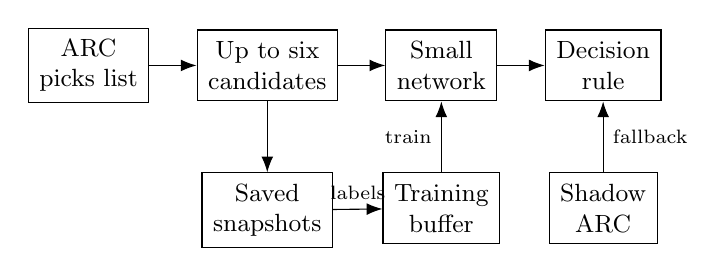
\begin{tikzpicture}[
  box/.style={draw, minimum height=0.9cm, align=center, font=\small, inner sep=4pt},
  arr/.style={-{Latex[length=2mm]}},
  node distance=0.9cm and 0.6cm
]
\node[box] (arc) {ARC\\picks list};
\node[box, right=of arc] (cand) {Up to six\\candidates};
\node[box, right=of cand] (net) {Small\\network};
\node[box, right=of net] (rule) {Decision\\rule};
\node[box, below=of cand] (pend) {Saved\\snapshots};
\node[box, below=of net] (buf) {Training\\buffer};
\node[box, below=of rule] (shadow) {Shadow\\ARC};
\draw[arr] (arc) -- (cand);
\draw[arr] (cand) -- (net);
\draw[arr] (net) -- (rule);
\draw[arr] (cand) -- (pend);
\draw[arr] (pend) -- node[above, font=\scriptsize]{labels} (buf);
\draw[arr] (buf) -- node[left, font=\scriptsize]{train} (net);
\draw[arr] (shadow) -- node[right, font=\scriptsize]{fallback} (rule);
\end{tikzpicture}
\caption{The parts of TIDE. ARC picks the list, the network ranks a few candidates, and a shadow copy of ARC decides when to hand control back.}
\label{fig:architecture}
\end{figure}

\subsection{Candidates}

For the list ARC has chosen, TIDE looks at up to six items:
\begin{itemize}
\item the four oldest items, where the oldest one is ARC's own choice;
\item the newest item, which is often the right one to drop on long loops, because it will not come back until the loop comes round again;
\item the item being requested, which lets TIDE serve it without storing it. We call this a bypass. It protects the cache from one-time scans.
\end{itemize}
The number of candidates never depends on the cache size.

\subsection{Features}
\label{sec:features}

TIDE keeps a short history for each item it has seen recently, including items that were removed, so it can recognise them when they come back. From this history it builds the twelve numbers in Table~\ref{tab:features}. Time values are scaled by the cache size in the same way as the target. None of the features look at the content of an item, so the design works with any kind of key.

\begin{table}[htbp]
\centering
\caption{The twelve features computed for each candidate.}
\label{tab:features}
\begin{tabular}{L{1.0cm}L{4.3cm}L{5.7cm}}
\toprule
No. & Feature & What it captures \\
\midrule
1 & Time since last request & Recency \\
2 to 4 & Last three gaps between requests & Regular patterns and loops \\
5 & Smoothed average gap & Typical return time \\
6 & Capped request count & Whether the item is new or repeat \\
7 to 9 & Three fading counters & Popularity over short, medium and long spans \\
10 & Total request count & Long term popularity \\
11 & Is this the requested item? & Marks the bypass option \\
12 & Is it in the frequency list? & ARC's own view of the item \\
\bottomrule
\end{tabular}
\end{table}

There is no feature for trend. An item that is gaining popularity already shows shorter gaps and a short term counter that is higher than its long term one, and the network can learn to read that.

\subsection{Neural Network Architecture}
\label{sec:model}

At the centre of TIDE is a deep feedforward neural network that turns the twelve input features of Sect.~\ref{sec:features} into a single reuse-time score. Rather than a single hidden layer, the network stacks three hidden layers of decreasing width, so that early layers can combine raw recency and frequency signals into intermediate representations and later layers can sharpen those representations into a final ranking score. This layered structure is what lets the network pick up on combinations of signals, such as a short recent gap together with a rising short-term counter, that no single input feature captures on its own.

\begin{figure}[htbp]
\centering
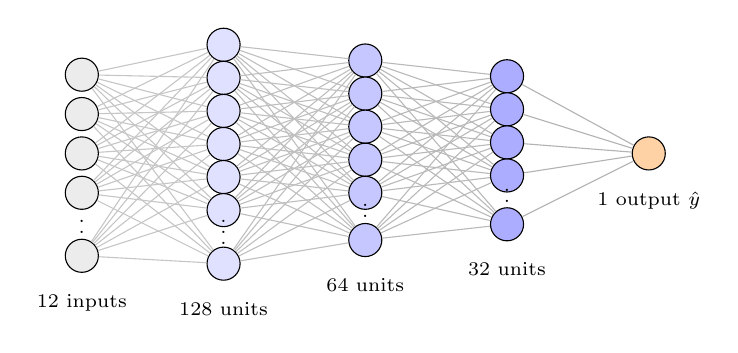
\begin{tikzpicture}[
  neuron/.style={circle, draw, minimum size=0.42cm, inner sep=0pt},
  lbl/.style={font=\scriptsize}
]
\foreach \i in {1,...,4} {\node[neuron, fill=gray!15] (i\i) at (0, -\i*0.5) {};}
\node[lbl] at (0,-2.4) {$\vdots$};
\node[neuron, fill=gray!15] (i5) at (0,-2.8) {};
\node[lbl, below=0.15cm of i5] {12 inputs};

\foreach \j in {1,...,6} {\node[neuron, fill=blue!12] (h1\j) at (1.8, -\j*0.42+0.3) {};}
\node[lbl] at (1.8,-2.4) {$\vdots$};
\node[neuron, fill=blue!12] (h17) at (1.8,-2.9) {};
\node[lbl, below=0.15cm of h17] {128 units};

\foreach \j in {1,...,5} {\node[neuron, fill=blue!22] (h2\j) at (3.6, -\j*0.42+0.1) {};}
\node[lbl] at (3.6,-2.2) {$\vdots$};
\node[neuron, fill=blue!22] (h26) at (3.6,-2.6) {};
\node[lbl, below=0.15cm of h26] {64 units};

\foreach \j in {1,...,4} {\node[neuron, fill=blue!32] (h3\j) at (5.4, -\j*0.42-0.1) {};}
\node[lbl] at (5.4,-2.0) {$\vdots$};
\node[neuron, fill=blue!32] (h35) at (5.4,-2.4) {};
\node[lbl, below=0.15cm of h35] {32 units};

\node[neuron, fill=orange!35] (o) at (7.2,-1.5) {};
\node[lbl, below=0.15cm of o] {1 output $\hat{y}$};

\foreach \i in {1,...,5} \foreach \j in {1,...,7} \draw[gray!45, thin] (i\i) -- (h1\j);
\foreach \i in {1,...,7} \foreach \j in {1,...,6} \draw[gray!50, thin] (h1\i) -- (h2\j);
\foreach \i in {1,...,6} \foreach \j in {1,...,5} \draw[gray!55, thin] (h2\i) -- (h3\j);
\foreach \i in {1,...,5} \draw[gray!60, thin] (h3\i) -- (o);
\end{tikzpicture}
\caption{The deep scoring network: three hidden layers with ReLU activations narrow twelve raw features down to one reuse-time score.}
\label{fig:network}
\end{figure}

\subsubsection{Input representation.}
Each candidate is represented by the twelve-dimensional feature vector $x \in \mathbb{R}^{12}$ described in Table~\ref{tab:features}. This plays the same role that an embedding layer plays in larger deep learning systems: it turns raw, irregularly scaled measurements (ages, gaps, counts) into a fixed-size numerical vector that a network layer can consume directly.

\subsubsection{Layer stack.}
The network computes
\begin{align}
h_1 &= \mathrm{ReLU}(W_1 x + b_1), & W_1 &\in \mathbb{R}^{128 \times 12},\\
h_2 &= \mathrm{ReLU}(W_2 h_1 + b_2), & W_2 &\in \mathbb{R}^{64 \times 128},\\
h_3 &= \mathrm{ReLU}(W_3 h_2 + b_3), & W_3 &\in \mathbb{R}^{32 \times 64},\\
\hat{y} &= w_4^\top h_3 + b_4, & w_4 &\in \mathbb{R}^{32},
\end{align}
with rectified linear activations between layers and a linear output head, giving roughly 12,000 trainable parameters across the four weight matrices. Figure~\ref{fig:network} shows the resulting architecture. Each hidden layer halves the width of the one before it, a common design pattern in deep networks that keeps early layers wide enough to preserve information from the raw features while letting later layers specialise toward the regression target.

\subsubsection{Training objective.}
The network is trained end to end by backpropagation to minimise the mean squared error between $\hat{y}$ and the transformed reuse-time target $g(d)$ of Eq.~(\ref{eq:target}). Because the true label for a candidate is only known once it is requested again or its window expires (Sect.~\ref{sec:online-training}), every training example is a form of delayed, weakly supervised signal, closer to the censored-regression problems studied in survival analysis than to a standard supervised dataset with labels available up front. The network nonetheless learns entirely through gradient descent on this loss, with no reward shaping and no trial-and-error exploration of the kind used in reinforcement learning.

The network is deliberately kept small in absolute terms, even though it is deep in structure: it is evaluated on at most six candidates per decision, so a wide, heavily over-parameterised network would add latency without adding useful representational power. The three-layer design is chosen to be the smallest depth at which the network can combine recency, frequency and periodicity signals nonlinearly, while still running well within a microsecond-scale latency budget.

\subsection{Decision Rule}

TIDE removes the candidate with the highest score, with one condition: any candidate other than ARC's own choice has to win by a margin. For the other old items the margin is 0.1, which means the model must expect the item to return roughly 10\% later than ARC's choice. For the newest item and the bypass option the margin is 0.2, or roughly 22\% later, because these moves are riskier. When the model is unsure, ARC's choice stands.

\subsection{Online Training}
\label{sec:online-training}

The network is trained continually, in an online, continual-learning setting rather than on a fixed offline dataset. Each time a candidate is scored, its feature vector is saved. When that item is requested again, the saved features get their true label. If the item has not come back after $W = 8c$ requests, it is labelled as ``far away'' instead. Labelled examples go into a replay buffer of 32,768 rows, the same kind of experience-replay mechanism used to stabilise training in deep reinforcement learning systems, and after every 32 new labels the network takes one stochastic gradient step on a random minibatch of 256 rows using the Adam optimiser~\cite{kingma2015}. Sampling minibatches at random from the buffer, rather than training on labels in the order they arrive, breaks the correlation between consecutive requests and keeps the gradient estimates stable. The network is not used to make decisions at all until at least 2,048 labels have been collected, so every early decision is ARC's and the network only takes over once it has seen enough examples to have learned a meaningful mapping from features to reuse time.

\subsection{Fallback}

A second copy of ARC, the shadow, sees the same requests and keeps only keys. TIDE counts its misses and the shadow's misses over windows of a few thousand requests. If TIDE misses clearly more in a window, it stops using the model and lets ARC decide for a while. The pause starts at two windows and doubles after each repeated failure, up to 32 windows. Training carries on during the pause. Table~\ref{tab:params} lists all settings. They are chosen before any testing and are the same for every workload.

\begin{table}[htbp]
\centering
\caption{Design settings, fixed in advance for all workloads.}
\label{tab:params}
\begin{tabular}{L{3.8cm}L{2.5cm}L{4.4cm}}
\toprule
Setting & Value & Reason \\
\midrule
Candidates per decision & Up to 6 & Keeps cost fixed \\
Label window $W$ & $8c$ & Covers several cache turnovers \\
Hidden layers & 128, 64, 32 & About 12,000 parameters in total \\
Training buffer & 32,768 rows & Old patterns fade out \\
Training step & Every 32 labels & Limits training time \\
Batch size & 256 & Stable updates \\
Margins & 0.1 and 0.2 & Model must be clearly better \\
Start after & 2,048 labels & No untrained decisions \\
Fallback window & $\max(2000, 4c)$ & Enough requests to compare \\
Fallback tolerance & 1\% of the window & Small losses are ignored \\
\bottomrule
\end{tabular}
\end{table}

\section{Theoretical Analysis}
\label{sec:analysis}

This section gives short arguments for how the design should behave. We assume that the cache does not change which items users request.

\subsection{Labels Come for Free}

Every scored candidate gets exactly one label within $W$ requests. The label depends only on when the item is requested again, not on what the cache did. This is the main difference from reinforcement learning. The cache never has to try bad moves to learn, and it never has to work out which of its past actions led to a later miss.

\subsection{Cost Stays Fixed}

A hit does not use the network at all. A miss runs a forward pass through the three-layer network for at most six candidates, which is about 71,000 multiply and add operations in total, still small enough to execute in a few microseconds on ordinary hardware. The replay buffer takes about 1.7 MB no matter how big the cache is, and the network and optimiser state together take well under a megabyte. Only the per item history grows with the cache, in the same way that ARC's ghost lists do. The cost of a decision therefore does not grow as the cache gets bigger, regardless of how deep the network is, since its depth is fixed in advance and never scales with cache size.

\subsection{Loops Longer Than the Cache}

Take a cache of 16 items and a workload that requests keys 1 to 17 in order, over and over. LRU always removes the item that is needed next, so it never hits. FIFO does the same, and so does ARC. Belady's rule misses once every 16 requests, which gives a hit rate of 93.75\%. A policy that keeps 16 keys fixed and never stores the 17th does even better: it misses once per round of 17 requests, for 94.1\%. No policy can beat that, because at least one of the 17 keys must miss in every round.

TIDE has both of the moves needed here. It can remove the newest item, which is what Belady's rule does, and it can skip storing the requested item, which is what the bypass policy does. ARC can do neither.

\subsection{When There Is Nothing to Learn}

If every request is picked at random from $N$ equally likely items, the chance of a hit is $c/N$ for any policy that keeps the cache full, because the next request has nothing to do with what is in the cache. TIDE cannot beat ARC here, and it should not lose either. When some items are more popular than others but requests are still random, the best possible policy keeps the most popular items~\cite{aho1971}. TIDE can only gain the difference between ARC and that best policy, which is usually small.

\subsection{How Far It Can Fall Behind ARC}

The fallback limits how much worse than ARC TIDE can be over a long run. Suppose the model keeps failing. After a few failures, each window in which the model is used is followed by 32 windows in which ARC decides, so at most about one window in 33 is lost. That caps the long run loss at about 3\% of ARC's hits. A workload that switches back and forth between fooling the model and suiting it perfectly could push the loss up to about a quarter of ARC's hits, because a single good window resets the pause. Requiring several good windows in a row before trusting the model again would close this gap. Both figures assume that once ARC is back in control, the two caches quickly end up holding similar items.

\section{Discussion}
\label{sec:expected}

Table~\ref{tab:predictions} sums up what the analysis suggests for different kinds of workload.

\begin{table}[htbp]
\centering
\caption{Expected gain of TIDE over ARC by workload type.}
\label{tab:predictions}
\begin{tabular}{L{2.6cm}L{3.5cm}L{1.7cm}L{2.6cm}}
\toprule
Workload & What helps & Expected gain & Why \\
\midrule
Uniform random & Nothing & None & No pattern to learn \\
Skewed random & Popularity counters & Small & Best rule is close to ARC \\
Loops & Newest item removal, bypass & Large & ARC gets no hits \\
Scans & Bypass & Moderate & Scan items are skipped \\
Phase changes & Relearning, fallback & Moderate & Losses are capped \\
Slow popularity drift & Gap and counter features & Small & Changes are gradual \\
Strong locality & Nothing & Near zero & LRU is already close to best \\
\bottomrule
\end{tabular}
\end{table}

The gain should depend on how much structure the workload has. With no pattern there is nothing to learn, and with very strong locality LRU is already close to the best possible. The largest gains should come where recency is misleading, as in loops and scans. For skewed random traffic, the gain should be largest at moderate skew, where recency and popularity disagree most often. For loops, the gain should be largest when the loop is just a little longer than the cache.

At the start of every workload TIDE behaves exactly like ARC, because the model waits for enough labels. After a sudden change in the workload, the model may make poor choices until the buffer fills with new examples, and the fallback limits the cost of that period. In a prototype written in Python, we expect a decision to take tens of microseconds, which is slower than native ARC but does not grow with the cache.

\section{Evaluation Methodology}
\label{sec:plan}

The expectations above can be tested. Table~\ref{tab:hypotheses} states them as hypotheses along with the result that would show each one to be wrong, and Table~\ref{tab:setup} describes the planned setup. All settings are fixed before any test is run.

\begin{table}[htbp]
\centering
\caption{Hypotheses to test.}
\label{tab:hypotheses}
\begin{tabular}{L{0.7cm}L{5.2cm}L{4.9cm}}
\toprule
& Hypothesis & Wrong if \\
\midrule
H1 & TIDE has the best average normalised hit rate & Any baseline matches or beats it \\
H2 & On loops, TIDE gets close to the bypass rate while ARC stays near zero & TIDE stays close to ARC \\
H3 & On uniform random traffic, TIDE and ARC tie & The gap is larger than run-to-run noise \\
H4 & TIDE never falls far behind ARC & Any case loses more than about one point \\
H5 & Decision time does not grow with cache size & Median decision time rises with the cache \\
\bottomrule
\end{tabular}
\end{table}

\begin{table}[htbp]
\centering
\caption{Planned test setup.}
\label{tab:setup}
\begin{tabular}{L{2.4cm}L{8.3cm}}
\toprule
Item & Plan \\
\midrule
Workloads & Uniform and skewed random traffic, loops, scans, bursty and periodic traffic, drifting popularity and sudden phase changes \\
Cache sizes & 0.1\%, 1\% and 10\% of the distinct keys in each workload \\
Baselines & LRU, LFU, ARC, S3-FIFO and SIEVE \\
Reference points & Belady's rule, and TIDE given the true reuse distances \\
Measures & Normalised hit rate, cases won, worst case against ARC, decision time and training time \\
Repeats & At least three runs with different seeds \\
\bottomrule
\end{tabular}
\end{table}

Running TIDE with the true reuse distances in place of the network shows how much of any shortfall comes from the choice of candidates and how much comes from the model.

\section{Limitations}
\label{sec:limits}

The loss bound assumes that TIDE and the shadow quickly hold similar items once ARC is back in control, which is only roughly true. The design also assumes that every item has the same size. Items that return after more than $W$ requests all get the same ``far away'' label, so the model cannot tell them apart. The candidates the model sees depend on its own earlier choices, so what it trains on may drift from what it is asked to judge. Finally, all settings are fixed in advance, and the design has no way to tune them for a given workload.

\section{Conclusion}
\label{sec:conclusion}

TIDE keeps ARC's choice of which list to shrink and hands the choice of which item to remove from it to a deep neural network, with the option of not caching a new item at all. The network is a three-hidden-layer architecture trained end to end by backpropagation, and because its training labels come from the request stream itself, replayed through an experience buffer, it can learn continually while the cache runs, with no offline data and no trial and error. The cost of each decision stays fixed regardless of the network's depth, and a shadow copy of ARC limits how much the network can hurt. We expect clear gains on loops, scans and phase changes, small gains on skewed random traffic, and none on uniform random traffic. The evaluation plan in Sect.~\ref{sec:plan} is designed to check each of these expectations.

\bibliographystyle{unsrt}
\bibliography{references}

\end{document}
